\documentclass[11pt]{amsart}
\usepackage[T1]{fontenc}
\usepackage{lmodern,microtype,amsmath,amssymb,mathtools,booktabs,array,tikz}
\usepackage[margin=1.05in]{geometry}
\usepackage[hidelinks]{hyperref}
\usetikzlibrary{arrows.meta,positioning,calc}
\raggedbottom
\setlength{\emergencystretch}{2em}
\newtheorem{theorem}{Theorem}[section]
\newtheorem{proposition}[theorem]{Proposition}
\newtheorem{lemma}[theorem]{Lemma}
\newtheorem{corollary}[theorem]{Corollary}
\theoremstyle{definition}
\newtheorem{definition}[theorem]{Definition}
\newtheorem{example}[theorem]{Example}
\newtheorem{remark}[theorem]{Remark}
\newcommand{\Q}{\mathbb Q}\newcommand{\C}{\mathbb C}\newcommand{\Z}{\mathbb Z}
\newcommand{\F}{\mathbb F}\newcommand{\Km}{\operatorname{Km}}
\newcommand{\Fix}{\operatorname{Fix}}\newcommand{\NS}{\operatorname{NS}}
\newcommand{\Num}{\operatorname{Num}}\newcommand{\Aut}{\operatorname{Aut}}
\newcommand{\tr}{\operatorname{tr}}\newcommand{\id}{\mathrm{id}}
\title[Involution geometry of product Kummer surfaces]{Explicit Involution Geometry of Product Kummer Surfaces}
\author{Deep Bhattacharjee}
\address{Electro--Gravitational Space Propulsion Laboratory (EGSPL), India}
\email{itsdeep@live.com}
\thanks{Deep Bhattacharjee is the corresponding author. ORCID: 0000-0003-0466-750X.}
\author{Pallab Nandi}
\address{Former student, Indian Institute of Science Education and Research Kolkata, India}
\email{pallabnandi995@gmail.com}
\subjclass[2020]{14J28, 14J50, 14K99}
\keywords{K3 surfaces, Kummer surfaces, Enriques surfaces, involutions}
\date{November 8, 2026. Revised review for Preprints.org, version 2.}
\begin{document}
\begin{abstract}
We classify the 31 nonidentity involutions in the standard affine two-torsion subgroup of a product Kummer surface. We compute their fixed loci, quotient surfaces and rational cohomology representations, including the fixed loci of all fifteen translations descending to each of the nine Lieberman quotients.
\end{abstract}
\maketitle
\section{Introduction and scope}
Let $E$ and $F$ be complex elliptic curves, let $A=E\times F$, and let
$X=\Km(A)$ be the minimal resolution of $A/\langle-1\rangle$.
The sixteen translations by points of $A[2]$ act on $X$. The reflection
$r(x,y)=(x,-y)$ acts as well. Together they form a particularly accessible
subgroup of $\Aut(X)$: every element is given by a formula on $A$, while
the exceptional curves can be tracked through the sixteen points of $A[2]$.

This article gives a complete calculation inside that subgroup. The
classification holds without a genericity assumption on $E$ and $F$.
Extra automorphisms may occur for special elliptic curves, but they do not
alter the fixed loci of the specified maps. We also calculate the action
on rational cohomology and the induced translations on the Enriques
quotients.\footnote{The nine free group elements need not give nine
pairwise nonisomorphic quotient surfaces for special choices of the
elliptic curves. No such isomorphism classification is used here.}
The proofs use the explicit local resolution, elementary
equations on elliptic curves, and finite-dimensional linear algebra.

The free involutions in this construction are the classical Lieberman
involutions. They are discussed explicitly by Ohashi \cite{Ohashi}.
Our classification concerns the indicated affine subgroup, not all
involutions of a Kummer surface. In particular, the nine free elements
below are not a classification of all Enriques quotients. A generic
product Kummer surface has fifteen distinct Enriques quotients up to
isomorphism \cite{Ohashi}. Counting elements of a group and counting
isomorphism classes of quotient surfaces are different tasks.

The paper replaces several inaccurate assertions in the earlier review
\cite{Previous}. A diagonal involution of the Fermat quartic that was
described as free has eight fixed points. A symplectic involution on a
general K3 surface has a K3 resolution as quotient, but the resolution need
not be Kummer. Positive Picard rank alone is not the projectivity
criterion. These distinctions are proved or explained in
Sections~\ref{sec:general}--\ref{sec:fermat} and Appendix~\ref{app:lattice}.
The revised title describes the explicit family treated here.

\subsection{Conventions}
All varieties and morphisms are over $\C$. A K3 surface means a smooth
projective surface with trivial canonical bundle and $H^1(\mathcal O)=0$.
An Enriques surface means a smooth projective surface with
$h^{1,0}=h^{2,0}=0$ and canonical bundle of exact order two. Intersection
forms are integral unless coefficients are stated. The lattice $U$ has
matrix $\left(\begin{smallmatrix}0&1\\1&0\end{smallmatrix}\right)$, and
$E_8(-1)$ is negative definite. We write $L(m)$ for a lattice with its
form multiplied by $m$. The elementary surface theory used below is
covered by Beauville \cite{Beauville} and Huybrechts \cite{Huybrechts}.

\subsection{The two principal statements}
Put $T=A[2]$, write $t_c$ for translation by $c$, and set
$G=\langle T,r\rangle$. In the following table, $a\in E[2]$ and
$b\in F[2]$.

\begin{theorem}\label{thm:classification}
The induced action identifies $G$ with $(\Z/2\Z)^5$. Its 31 nonidentity
elements have the following fixed loci on $X$.
\begin{center}
\begin{tabular}{@{}llll@{}}\toprule
Element & Condition & Number & Fixed locus\\\midrule
$t_c$ & $c\ne0$ & 15 & eight points\\
$rt_{(a,b)}$ & $a\ne0$, $b\ne0$ & 9 & empty\\
$rt_{(a,0)}$ & $a\ne0$ & 3 & two copies of $F$\\
$rt_{(0,b)}$ & $b\ne0$ & 3 & two copies of $E$\\
$r$ & & 1 & eight rational curves\\\bottomrule
\end{tabular}
\end{center}
The translations are symplectic and the other sixteen elements are
antisymplectic. Resolving $X/\langle t_c\rangle$, for $c\ne0$, gives
$\Km(A/\langle c\rangle)$. Each of the nine free quotients is Enriques.
\end{theorem}

\begin{theorem}\label{thm:descent-intro}
Fix $a\ne0$ and $b\ne0$, set $\sigma=rt_{(a,b)}$, and let
$S=X/\langle\sigma\rangle$. All sixteen translations descend faithfully
to $S$. Every nonidentity descended translation has four isolated fixed
points. Among these fifteen maps, one has four additional rational
curves, two have two additional elliptic curves, four have one additional
elliptic curve, and eight have no fixed curve. The element associated
with $(a,b)$ acts trivially on $H^2(S,\Q)$; each of the other fourteen
has trace two.
\end{theorem}

The fixed-point calculations prove these statements for every product
$E\times F$. The accompanying exact-arithmetic program checks the finite
group bookkeeping and character multiplicities. It is a check of the
finite combinatorics, not a replacement for the geometric arguments.

\section{Constructing the Kummer surface}
\subsection{The sixteen singular points}
Write $\kappa(p)=-p$. The fixed locus of $\kappa$ on $A$ is $A[2]$,
which has sixteen points. At any such point choose analytic coordinates
$(z,w)$ in which $\kappa(z,w)=(-z,-w)$. The invariant local coordinates
$z^2,zw,w^2$ satisfy one relation,
\[
 (zw)^2=z^2w^2.
\]
Thus the quotient has an ordinary double point of type $A_1$. Away from
these points the quotient map is an unramified double covering.

Let $b:\widetilde A\to A$ be the blowup of the sixteen points. In one
blowup chart write $z=u,w=uv$. The lifted involution acts by
\[
 (u,v)\longmapsto(-u,v).
\]
The quotient has coordinates $(t,v)=(u^2,v)$ and is smooth. The other
chart gives the same conclusion. It follows that
\[
 X=\widetilde A/\langle\kappa\rangle
\]
is the minimal resolution of $A/\langle\kappa\rangle$.
Each exceptional curve on $X$ is a rational curve of self-intersection
$-2$. Indeed, the exceptional curve on $\widetilde A$ has square $-1$;
its pullback as a divisor from $X$ is twice that curve. The degree-two
intersection formula therefore gives $2C^2=4(-1)$.

\begin{figure}[tb]
\centering
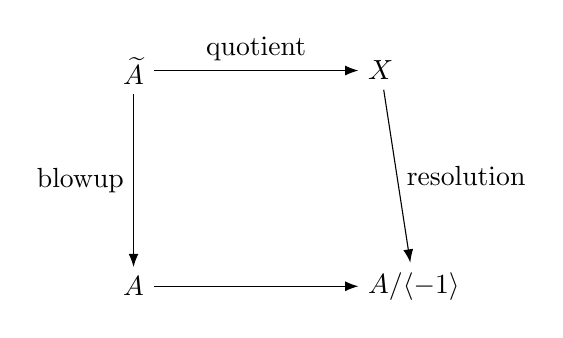
\begin{tikzpicture}[>=Latex,node distance=22mm and 26mm]
\node (At) {$\widetilde A$};\node[right=of At] (X) {$X$};
\node[below=of At] (A) {$A$};\node[right=of A] (Q) {$A/\langle-1\rangle$};
\draw[->] (At)--node[above]{quotient}(X);
\draw[->] (At)--node[left]{blowup}(A);
\draw[->] (A)--(Q);\draw[->] (X)--node[right]{resolution}(Q);
\end{tikzpicture}
\caption{The smooth Kummer model. The upper horizontal map is branched
along sixteen exceptional curves. The lower quotient has sixteen nodes.}
\label{fig:kummer}
\end{figure}

\subsection{The two-form and the invariants}
Choose nonzero holomorphic one-forms on $E$ and $F$. Their exterior
product $\omega$ is nowhere zero on $A$ and invariant under $\kappa$.
In the coordinates just used,
\[
 dz\wedge dw=u\,du\wedge dv=\frac12\,dt\wedge dv.
\]
Consequently the descended two-form extends across the exceptional
curve without a zero. This proves $K_X\simeq\mathcal O_X$ directly.

Blowing up points does not change $H^1(\mathcal O)$. The involution
$\kappa$ acts as $-1$ on $H^1(A,\mathcal O_A)$, so its invariant part
vanishes. Taking invariants under a finite group in characteristic zero
is exact; applying this to the finite quotient shows
$H^1(X,\mathcal O_X)=0$. Projectivity follows from the projective
blowup and finite quotient. Hence $X$ is K3.

The Euler characteristic of $A$ is zero. Each point blowup adds one, so
$e(\widetilde A)=16$. The fixed locus of the lifted $\kappa$ is the
disjoint union of sixteen projective lines and has Euler characteristic
$32$. The elementary Euler formula for an involution gives
\[
 e(X)=\frac{16+32}{2}=24.
\]
Since $b_1=b_3=0$, it follows that $b_2=22$.

\begin{remark}
The local calculation is also why the singular quotient and its smooth
resolution must not be interchanged. A line bundle pulled back from the
singular quotient has intersection zero with a contracted exceptional
curve, so that pullback cannot be ample on the resolution.
\end{remark}

\section{The affine two-torsion subgroup}
\subsection{Descent and faithfulness}
For $c\in T$, the equality $2c=0$ implies $t_c\kappa=\kappa t_c$.
Also $r\kappa=\kappa r$. These maps permute the centers of the blowup
and therefore lift to $\widetilde A$ and descend to $X$.
On $T$, the reflection $r$ is the identity. Hence $r$ commutes with all
$t_c$, and all resulting elements have order at most two.

No nonzero translation induces the identity on $X$. If it did, then on
the complement of the nodes one would have $p+c=p$ or $p+c=-p$ for
every $p$. The first equality forces $c=0$; the second describes only
the finite set $2p=-c$. Similarly, a map $rt_c$ cannot induce the
identity: neither $rt_c=p$ nor $rt_c=-p$ can hold on an open subset
of the two-dimensional abelian surface. Thus the 32 maps are distinct.

Translations preserve $\omega$, whereas $r^*\omega=-\omega$. Their
symplectic types are unchanged on passing to $X$.

\subsection{Fixed points of a translation}
\begin{proposition}\label{prop:translation}
For $c\ne0$, $\Fix_X(t_c)$ consists of eight points outside the
exceptional curves. The derivative at each of these points is $-I$.
\end{proposition}
\begin{proof}
A nonexceptional point of $X$ is the orbit $\{p,-p\}$. It is fixed
precisely when $p+c=p$ or $p+c=-p$. The first alternative is impossible.
The second is $2p=-c=c$. Multiplication by two on a complex abelian
surface has degree sixteen, so it has sixteen solutions. None belongs
to $A[2]$, since $c\ne0$. Pairing $p$ with $-p$ leaves eight orbits.
Translation acts on $A[2]$ without a fixed point, so it fixes no
exceptional curve or point on such a curve.

Near a solution, identify the neighborhood of $-p$ with that of $p$
using inversion. The composite with translation then has derivative
$-I$. In particular all eight points are isolated and nondegenerate.
\end{proof}

\begin{proposition}\label{prop:quotient}
Let $B=A/\langle c\rangle$, $c\ne0$. The minimal resolution of
$X/\langle t_c\rangle$ is $\Km(B)$.
\end{proposition}
\begin{proof}
The commuting actions yield an isomorphism of normal quotient surfaces
\[
 A/\langle\kappa,t_c\rangle
   \simeq (A/\langle c\rangle)/\langle-1\rangle.
\]
The surface $B$ is abelian, since the translation quotient is a finite
isogeny. Its Kummer resolution is smooth with trivial canonical bundle
by the calculation of Section 2. The quotient $X/\langle t_c\rangle$
has only the eight $A_1$ singularities of
Proposition~\ref{prop:translation}; its resolution also has trivial
canonical bundle and $h^{1,0}=0$. Both smooth resolutions are birational
to the displayed normal quotient. Smooth minimal K3 surfaces that are
birational are isomorphic: a birational map between smooth surfaces
factors into point blowups and blowdowns, whereas a K3 surface has no
$(-1)$-curve by adjunction. This proves the assertion.
\end{proof}

The product hypothesis enters the reflection calculation below, but not
Proposition~\ref{prop:quotient}. In particular $B$ need not itself be a
product of elliptic curves.

\section{The sixteen antisymplectic involutions}
Set $\sigma_{a,b}=rt_{(a,b)}$. On $A$ this is
\[
 (x,y)\longmapsto(x+a,-y+b).
\]
For a point outside $A[2]$, its orbit in the quotient is fixed exactly
when one of the following equations holds:
\begin{align}
 \sigma_{a,b}(x,y)=(x,y)
   &\quad\Longleftrightarrow\quad a=0,\quad 2y=b,\label{eq:plus}\\
 \sigma_{a,b}(x,y)=(-x,-y)
   &\quad\Longleftrightarrow\quad b=0,\quad 2x=a.\label{eq:minus}
\end{align}
These two equations exhaust the possibilities, since the quotient orbit
has only two elements.

\subsection{Both translation components nonzero}
If $a$ and $b$ are nonzero, neither equation can hold. On the sixteen
nodes, $\sigma_{a,b}$ acts as translation by $(a,b)$, so it pairs the
nodes and their exceptional curves without a fixed point. Therefore
$\sigma_{a,b}$ is free on all of $X$. There are $3\cdot3=9$ choices.

\subsection{Exactly one translation component nonzero}
Suppose $a\ne0$ and $b=0$. Equation~\eqref{eq:minus} gives four roots
of $2x=a$, and $y$ is arbitrary. None of these $x$ lies in $E[2]$.
Inversion pairs the four roots into two pairs. On each pair of copies
of $F$, the quotient by inversion is isomorphic to one copy of $F$:
choosing one root identifies that component with $F$, and the other
root is its inverted partner. Thus the fixed locus consists of two
disjoint smooth elliptic curves. No exceptional curve is fixed, since
the nodes are translated by the nonzero point $(a,0)$.
The case $a=0,b\ne0$ follows from Equation~\eqref{eq:plus} and gives
two copies of $E$.

\subsection{The reflection itself}
For $a=b=0$, Equations~\eqref{eq:plus}--\eqref{eq:minus} give
\[
 E\times F[2]\quad\text{and}\quad E[2]\times F.
\]
After quotienting by inversion, each of these eight elliptic curves
becomes a projective line. Their proper transforms on $X$ are disjoint.
At a crossing, the two branches meet the exceptional curve at distinct
points, separating the proper transforms.

To check that no further fixed point has been missed, use local
coordinates with $r(z,w)=(z,-w)$. In the blowup chart $z=u,w=uv$,
the action is $(u,v)\mapsto(u,-v)$. On the quotient chart
$(t,v)=(u^2,v)$ it remains $(t,v)\mapsto(t,-v)$. The exceptional
curve $t=0$ has one fixed point in this chart, $v=0$, already belonging
to the proper transform of $w=0$. The other chart gives the other
fixed point, on the proper transform of $z=0$. There are no isolated
fixed points left over.

\begin{figure}[tb]
\centering
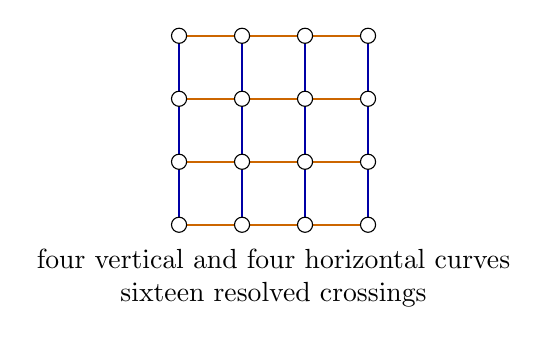
\begin{tikzpicture}[scale=.8]
\foreach \x in {0,1,2,3}{\draw[blue!65!black,thick] (\x,0)--(\x,3);}
\foreach \y in {0,1,2,3}{\draw[orange!80!black,thick] (0,\y)--(3,\y);}
\foreach \x in {0,1,2,3}{\foreach \y in {0,1,2,3}{\fill[white] (\x,\y) circle (.12);\draw (\x,\y) circle (.12);}}
\node[align=center] at (1.5,-.85) {four vertical and four horizontal curves\\sixteen resolved crossings};
\end{tikzpicture}
\caption{Incidence schematic of the double Kummer configuration.
Each small circle represents an exceptional curve, not a remaining
intersection of the eight fixed rational curves.}
\label{fig:grid}
\end{figure}

\subsection{The Enriques quotients}
Let $\sigma=\sigma_{a,b}$ with $a,b\ne0$. The map $\pi:X\to S=X/\sigma$
is an unramified double covering of smooth projective surfaces. Since
$\sigma$ acts by $-1$ on $H^0(X,K_X)$, we have $h^{2,0}(S)=0$.
Also $H^1(S,\mathcal O_S)$ injects into $H^1(X,\mathcal O_X)=0$.
The covering formula gives $\pi^*K_S=K_X=0$; taking the norm gives
$K_S^{\otimes2}\simeq\mathcal O_S$. It is not trivial, since otherwise
$h^{2,0}(S)=1$. Hence $S$ is Enriques.

The topological covering gives $e(S)=12$, and Hodge theory gives
$b_1=b_3=0$, so $b_2(S)=10$. For divisor classes $D,D'$,
\begin{equation}\label{eq:intersection}
 (\pi^*D,\pi^*D')_X=2(D,D')_S.
\end{equation}
The same formula holds for rational degree-two cohomology classes.
\footnote{The factor two is the degree of the unramified covering. It
must be retained when comparing the Enriques numerical lattice with
its pullback in the K3 lattice.}
This finishes the geometric proof of
Theorem~\ref{thm:classification}.

\section{The rational cohomology representation}
\subsection{Cohomology through the resolution}
There is a $G$-equivariant rational decomposition
\begin{equation}\label{eq:H2}
 H^2(X,\Q)\simeq H^2(A,\Q)\oplus\bigoplus_{v\in T}\Q e_v.
\end{equation}
One way to see it is to apply the blowup formula on $\widetilde A$.
The lifted $\kappa$ acts trivially on $H^2(A,\Q)$, because it acts as
$-1$ on $H^1(A,\Q)$, and it fixes every exceptional class. Rational
cohomology of a finite quotient identifies with the invariant
cohomology of the covering space. The latter statement follows, for
example, by averaging cochains after a compatible triangulation; the
averaging operator is available because the group order is invertible
in $\Q$. This yields \eqref{eq:H2}.

Translations act trivially on $H^2(A,\Q)$ and regularly permute the
sixteen $e_v$. The K\"unneth decomposition is
\[
 H^2(A,\Q)=H^2(E,\Q)\oplus
   \bigl(H^1(E,\Q)\otimes H^1(F,\Q)\bigr)\oplus H^2(F,\Q).
\]
The reflection has signs $+,-,+$ on these three terms, of dimensions
$1,4,1$. It fixes the exceptional classes.

\begin{proposition}\label{prop:character}
Let $\widehat T=\operatorname{Hom}(T,\{\pm1\})$. Write
$\Q_{\chi,\epsilon}$ for the character on which $t_c$ acts by
$\chi(c)$ and $r$ acts by $\epsilon$. Then
\[
 H^2(X,\Q)\simeq
 \Q_{1,+}^{\,3}\oplus\Q_{1,-}^{\,4}
       \oplus\bigoplus_{\substack{\chi\in\widehat T\\\chi\ne1}}
                  \Q_{\chi,+}.
\]
\end{proposition}
\begin{proof}
The regular representation of the elementary abelian group $T$ is the
sum of its sixteen rational characters, each once. The reflection acts
as $+1$ on that entire summand. The K\"unneth calculation contributes
two trivial characters with sign $+$ and four with sign $-$. Adding
these contributions proves the formula; the dimensions sum to 22.
\end{proof}

\begin{corollary}\label{cor:traces}
The traces on $H^2(X,\Q)$ are $6$ for $t_c$, $c\ne0$, $14$ for $r$,
and $-2$ for $rt_c$, $c\ne0$. The corresponding invariant dimensions
are $14,18,10$.
\end{corollary}
\begin{proof}
A nonidentity translation has trace zero on the regular summand and
trace six on $H^2(A)$. The reflection has trace $16+2-4=14$.
Combining a nonzero translation with the reflection gives $0+2-4=-2$.
For an involution on a 22-dimensional space, the invariant dimension is
$(22+\tr)/2$.
\end{proof}

The topological Lefschetz formula reads $e(\Fix(g))=2+\tr(g|H^2)$.
It gives respectively $8,16,0$, agreeing with all of the fixed loci
above. In particular the elliptic fixed curves and the empty fixed
locus have the same Euler characteristic. A trace calculation alone
does not distinguish them; the geometric equations are necessary.

\section{Translations on a Lieberman quotient}\label{sec:descent}
Fix nonzero $a\in E[2]$, $b\in F[2]$, and put $c_0=(a,b)$,
$\sigma=rt_{c_0}$, $S=X/\sigma$. Every translation commutes with
$\sigma$ and induces an automorphism $\overline t_c$ of $S$.
The descended action is faithful: the kernel on $X$ would have to be
contained in the deck group $\{1,\sigma\}$, but no translation equals
the antisymplectic map $\sigma$.

\subsection{Lifting the fixed locus}
For any $c\ne0$,
\begin{equation}\label{eq:fixedlift}
 \pi^{-1}\Fix_S(\overline t_c)
       =\Fix_X(t_c)\sqcup\Fix_X(\sigma t_c).
\end{equation}
The union is disjoint: a point fixed by both would be fixed by
$\sigma$, contrary to freeness. Each set is $\sigma$-stable. The
first contains eight points, paired freely by $\sigma$, and therefore
gives four isolated points on $S$. They are nondegenerate because the
local derivative is $-I$. Any fixed curve comes from the second set.
Now
\[
 \sigma t_c=rt_{c_0+c}.
\]
Thus the previous classification reduces the calculation to the
pairing of the relevant elliptic or rational curves.

\begin{theorem}\label{thm:descent}
Besides four isolated points, the fixed locus of $\overline t_c$ has
the following curves. Every entry is a disjoint union.
\begin{center}
\begin{tabular}{@{}lll@{}}\toprule
$c$ & Number of choices & Fixed curves on $S$\\\midrule
$(a,b)$ & 1 & four copies of $\mathbb P^1$\\
$(a,0)$ & 1 & two copies of $E/\langle a\rangle$\\
$(0,b)$ & 1 & two copies of $F/\langle b\rangle$\\
$(a,d)$, $d\notin\{0,b\}$ & 2 & one copy of $E$\\
$(d,b)$, $d\notin\{0,a\}$ & 2 & one copy of $F$\\
all other nonzero $c$ & 8 & none\\\bottomrule
\end{tabular}
\end{center}
\end{theorem}
\begin{proof}
For $c=c_0$, the second set in \eqref{eq:fixedlift} is the eight
rational curves fixed by $r$. The map $\sigma$ translates their
two-torsion indices by $b$ or $a$, so it pairs them into four pairs.
Each pair descends to one rational curve.

For $c=(a,0)$, the second set is the fixed locus of $rt_{(0,b)}$,
namely two copies of $E$. They arise from the four roots of $2y=b$,
paired by inversion. On these roots, $-y+b=y$, because $2y=b$.
Hence $\sigma$ preserves each resulting elliptic curve and acts on it
by $x\mapsto x+a$. The quotient is $E/\langle a\rangle$.
The case $c=(0,b)$ is obtained by interchanging the factors and gives
two copies of $F/\langle b\rangle$.

For $c=(a,d)$ with $d\notin\{0,b\}$, the second set consists of two
copies of $E$, indexed by the roots of $2y=b+d$ modulo sign.
The operation $y\mapsto-y+b$ exchanges the two pairs. Indeed it could
preserve a pair only if $-y+b=y$ or $-y+b=-y$, requiring respectively
$2y=b$ or $b=0$, both impossible. Thus $\sigma$ exchanges the two
elliptic curves, and their image is one curve isomorphic to $E$.
The fourth family is symmetric and gives one copy of $F$.

There remain eight nonzero $c$ for which both components of $c_0+c$
are nonzero. The map $\sigma t_c$ is then free, so it adds no curve.
The list has $1+1+1+2+2+8=15$ elements and is exhaustive.
\end{proof}

\subsection{The numerical representation}
\begin{corollary}\label{cor:numerical}
The kernel of the translation action on $H^2(S,\Q)$ is
$\{0,c_0\}$. With $\overline T=T/\langle c_0\rangle$, the faithful
representation is
\[
 H^2(S,\Q)\simeq \Q^3\oplus
       \bigoplus_{\substack{\chi\in\widehat{\overline T}\\\chi\ne1}}\Q_\chi.
\]
Every nonidentity element of $\overline T$ has trace two and
six-dimensional invariant subspace. The map $\overline t_{c_0}$ is
numerically trivial, although it is not the identity automorphism.
\end{corollary}
\begin{proof}
The pullback identifies $H^2(S,\Q)$ with the $\sigma$-invariants in
\eqref{eq:H2}. In the $H^2(A)$ summand only the two factor classes
survive. Among the sixteen exceptional characters, precisely the
eight with $\chi(c_0)=1$ survive. They form the regular representation
of $\overline T$. This proves the decomposition and its kernel.
Alternatively, the special fixed locus has Euler characteristic
$4\cdot2+4=12$, giving trace ten; all other fixed loci have Euler
characteristic four, giving trace two.
Since $h^{2,0}(S)=0$, the rational second cohomology is algebraic by
the integral $(1,1)$ theorem, so triviality on rational cohomology is
triviality on the numerical divisor space. Its integral lattice is
torsion-free; a rationally trivial integral action is the identity.
\end{proof}

\begin{figure}[tb]
\centering
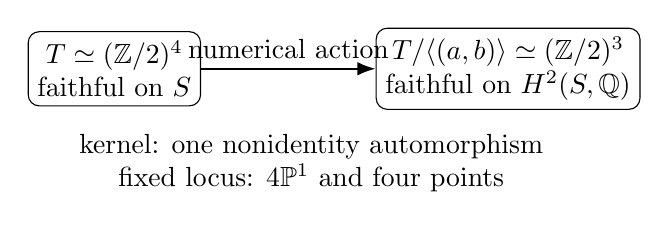
\begin{tikzpicture}[>=Latex,every node/.style={align=center}]
\node[draw,rounded corners] (T) at (0,0) {$T\simeq(\Z/2)^4$\\faithful on $S$};
\node[draw,rounded corners] (N) at (5,0) {$T/\langle(a,b)\rangle\simeq(\Z/2)^3$\\faithful on $H^2(S,\Q)$};
\draw[->,thick] (T)--node[above]{numerical action}(N);
\node at (2.5,-1.2) {kernel: one nonidentity automorphism\\fixed locus: $4\mathbb P^1$ and four points};
\end{tikzpicture}
\caption{Faithfulness on the surface differs from faithfulness on its
numerical divisor space. Both kernels are computed explicitly.}
\end{figure}

\section{General K3 involutions and the Kummer distinction}\label{sec:general}
The explicit construction illustrates a general local dichotomy but
does not remove the hypotheses of that dichotomy.

\begin{proposition}\label{prop:local}
A nonidentity symplectic involution of a complex K3 surface has eight
isolated fixed points. An antisymplectic involution has only smooth
fixed curves, or has empty fixed locus.
\end{proposition}
\begin{proof}
Finite-order analytic actions are locally linearizable by averaging
coordinates. At a fixed point the eigenvalues are $\pm1$. A
symplectic action has determinant one. If both eigenvalues are $+1$,
linearization makes the automorphism locally, hence globally, the
identity. Thus a nonidentity symplectic involution has derivative
$-I$ at every fixed point. Its holomorphic Lefschetz number on
$\mathcal O$ is $1+1=2$; each such point contributes
$1/\det(I-(-I))=1/4$. There are eight points.

An antisymplectic action has determinant $-1$, so the eigenvalues are
$1,-1$. Its fixed set is locally the smooth $+1$ eigendirection.
Different fixed components cannot cross, because the local fixed set
is a single smooth curve.
\end{proof}

The holomorphic Lefschetz theorem is used here in its standard
surface form, not reproved. The product calculation of the eight
translation fixed points in Proposition~\ref{prop:translation} did not
need it.

\begin{proposition}\label{prop:notkummer}
The resolution of the quotient of a K3 surface by a symplectic
involution is K3. It need not be Kummer.
\end{proposition}
\begin{proof}
The quotient has eight $A_1$ singularities. The local resolution
extends the invariant two-form without zeros, exactly as in Section 2.
Invariant $H^1(\mathcal O)$ vanishes, proving the K3 assertion.

For the second assertion, projective K3 surfaces with a symplectic
involution and Picard number nine exist; the families and their
lattices are described by van Geemen and Sarti \cite{vGS}.
The quotient resolution has the same transcendental rank: the
degree-two quotient correspondence identifies the transcendental
rational Hodge structures, with the intersection form rescaled.
Indeed a symplectic involution acts trivially on the transcendental
part, since its negative eigenspace is of type $(1,1)$ and therefore
algebraic. Consequently both K3 surfaces have Picard number nine.
Every projective Kummer surface has Picard number at least seventeen:
the sixteen independent exceptional classes are algebraic, and a
pulled-back polarization adds one more independent positive-square
class. The Picard-nine quotient is therefore not Kummer.
\end{proof}

The use of the cited Picard-nine family is essential to this
counterexample. The explicit product construction, by contrast, has
enough additional geometry to identify its translation quotients as
Kummer surfaces in Proposition~\ref{prop:quotient}.

\section{The Fermat quartic example corrected}\label{sec:fermat}
Consider the smooth quartic
\[
 Y=\{x_0^4+x_1^4+x_2^4+x_3^4=0\}\subset\mathbb P^3
\]
and the projective involution
\[
 \iota[x_0:x_1:x_2:x_3]=[-x_0:-x_1:x_2:x_3].
\]
A projective fixed point is an eigenline of the diagonal matrix.
The two eigenspaces are the lines
$L_-:\ x_2=x_3=0$ and $L_+:\ x_0=x_1=0$.
Their intersections with $Y$ are respectively
\[
 [z:1:0:0],\qquad[0:0:z:1],\qquad z^4=-1.
\]
The polynomial $z^4+1$ has four distinct roots because it has no
common root with $4z^3$. Thus $\iota$ has exactly eight fixed points.

The holomorphic two-form of a smooth quartic is the residue of the
standard homogeneous three-form divided by the defining polynomial.
The latter is invariant and the diagonal transformation has determinant
$+1$, so $\iota$ is symplectic. Its quotient resolution is K3 and is
not a free Enriques quotient. This corrects the earlier example
without changing the free Lieberman construction.

\begin{figure}[tb]
\centering
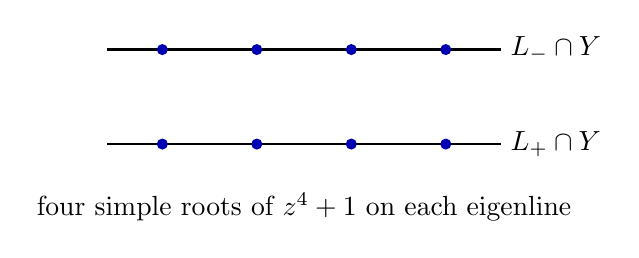
\begin{tikzpicture}[>=Latex]
\draw[thick] (0,0)--(5,0);\draw[thick] (0,1.2)--(5,1.2);
\foreach \x in {.7,1.9,3.1,4.3}{\fill[blue!70!black] (\x,0) circle(2pt);\fill[blue!70!black] (\x,1.2) circle(2pt);}
\node[right] at (5,0) {$L_+\cap Y$};\node[right] at (5,1.2) {$L_-\cap Y$};
\node[align=center] at (2.5,-.8) {four simple roots of $z^4+1$ on each eigenline};
\end{tikzpicture}
\caption{The diagram records two disjoint projective eigenlines and
their eight intersection points. It is an incidence schematic rather
than a spatial embedding of the quartic surface.}
\end{figure}

\section{Projective and lattice consequences}
For a complex K3 surface, projectivity is equivalent to the existence
of an integral $(1,1)$ class with positive square
\cite{Huybrechts}. Merely requiring a nonzero N\'eron--Severi group
is insufficient: a nonprojective K3 surface can have a negative-definite
or degenerate N\'eron--Severi lattice.
If $L$ is ample, a sufficiently high power is very ample; $L$ itself
need not define an embedding. In particular the existence of a
polarization must not be turned into an arbitrary quartic model.

The Kummer quotient $A/\langle-1\rangle$ can be singular even when
an associated linear system realizes it projectively. Its smooth
resolution contains sixteen $(-2)$-curves. A divisor giving a
contraction has zero intersection with those curves, and is nef
rather than ample on the resolution. The behavior of a product
principal polarization also differs from that of an indecomposable
principally polarized abelian surface. None of the arguments in this
paper requires a quartic embedding of the product Kummer surface.

For completeness, the standard integral lattice identifications used
for comparison are recorded in Appendix~\ref{app:lattice}. Our
rational character decomposition does not require their integral
classification. This separation prevents an unnoticed finite-index
issue from entering the fixed-locus calculation.

\section{Exact checks and reproducibility}
The file \texttt{checks/verify.py} uses only Python's standard library.
It models $T$ as $\F_2^4$ and $G$ as $\F_2^5$, lists all 31
nonidentity elements, and checks the counts in
Theorem~\ref{thm:classification}. It computes traces independently
from the permutation of the sixteen node labels and from the
character table. For each of the nine possible $c_0$, it checks the
15-case descent table and the multiplicity formula on $S$.

The geometric proof applies to every elliptic curve, whereas the
program checks its finite combinatorial shadow. It does not solve
equations numerically on a chosen elliptic curve, infer freeness from
sampling, or claim a formalization in a proof assistant.
The Fermat root check is exact: the Euclidean algorithm for
$z^4+1$ and $4z^3$ gives constant greatest common divisor.

\appendix
\section{Local quotient coordinates and fixed curves}\label{app:local}
It is useful to keep three maps separate. On $A$ the inversion has
isolated fixed points. On the blown-up surface $\widetilde A$ its
lift fixes each exceptional curve pointwise. On $X$ that exceptional
curve is the branch image and has self-intersection $-2$.
These different fixed sets belong to different surfaces.

In the first blowup chart $z=u,w=uv$, inversion is
$(u,v)\mapsto(-u,v)$ and the quotient is $(t,v)=(u^2,v)$.
In the second chart $z=sw,w=w$, the quotient is
$(s,q)=(s,w^2)$. The transition is
\[
 s=v^{-1},\qquad q=t v^2.
\]
The exceptional curve has normal transition $q=t v^2$, the transition
of $\mathcal O_{\mathbb P^1}(-2)$ under the corresponding coordinate
convention. The two-form patches agree because
\[
 \frac12\,dt\wedge dv=-\frac12\,dq\wedge ds.
\]
This is the complete local resolution of the ordinary double point.

For the reflection $(z,w)\mapsto(z,-w)$, the quotient coordinates
give $(t,v)\mapsto(t,-v)$ in the first chart and
$(s,q)\mapsto(-s,q)$ in the second. The two exceptional fixed points
are $v=0$ and $s=0$. They lie on the strict transforms of the two
coordinate axes, respectively. This proves both disjointness of the
eight rational fixed curves and the absence of additional isolated
points for $r$.

\section{Integral lattices and the rational calculation}\label{app:lattice}
The following are standard integral lattice theorems; they are
background, not claimed as new proofs here \cite{Huybrechts,vGS,Ohashi}:
\begin{align*}
 H^2(X,\Z)&\simeq U^{\oplus3}\oplus E_8(-1)^{\oplus2},\\
 H^2(X,\Z)^\nu&\simeq U^{\oplus3}\oplus E_8(-2)
       &&\text{for a symplectic involution }\nu,\\
 H^2(X,\Z)^{-\nu}&\simeq E_8(-2),\\
 \Num(S)&\simeq U\oplus E_8(-1),\\
 H^2(X,\Z)^\sigma&\simeq U(2)\oplus E_8(-2)
       &&\text{for a free involution }\sigma.
\end{align*}
The ranks in these formulas are $22$, $14$, $8$, $10$ and $10$.
They agree with the independently derived traces in
Corollary~\ref{cor:traces}. The factor two for the free quotient also
agrees with \eqref{eq:intersection}.

For a projective K3 surface, let $T_X=\NS(X)^\perp$. Orthogonality
gives
\[
 H^2(X,\Q)=\NS(X)_\Q\oplus T_{X,\Q}.
\]
Over $\Z$, the inclusion $\NS(X)\oplus T_X\subset H^2(X,\Z)$ usually
has a nontrivial finite cokernel. Discriminant forms supply the gluing.
Thus a rational direct-sum calculation cannot be promoted to an
integral orthogonal decomposition without checking that gluing.

Similarly, \eqref{eq:H2} is a rational $G$-module statement. It makes
no assertion that the sixteen exceptional classes and a chosen
integral copy of $H^2(A,\Z)$ form the entire integral K3 lattice.
Their primitive closure contains additional classes.

\section{An explicit enumeration of the descent cases}
Choose bases for $E[2]$ and $F[2]$ and write their elements as
$0,1,2,3$ with addition given by bitwise exclusive-or. Because any
nonzero vector in $\F_2^2$ can be sent to any other by a basis
change, it suffices for the combinatorial list to take $a=b=1$.
The special cases are
\[
 (1,1),\quad(1,0),\quad(0,1),\quad(1,2),\ (1,3),\quad
 (2,1),\ (3,1).
\]
They give respectively four rational curves, two elliptic curves,
two elliptic curves, and one elliptic curve for each of the last
four elements. The remaining nonzero elements are
\[
 (0,2),(0,3),(2,0),(3,0),(2,2),(2,3),(3,2),(3,3).
\]
For each of them both components of $c+c_0$ are nonzero. This list
also shows directly why there are eight curve-free cases.

For a character $\chi:T\to\{\pm1\}$, the projector
\[
 P_\chi=\frac1{16}\sum_{c\in T}\chi(c)t_c^*
\]
has rank three for the trivial character and rank one for each
nontrivial character on the reflection-positive part of $H^2(X)$.
On the reflection-negative part the trivial character has rank four
and all other projectors have rank zero. Imposing $\sigma$-invariance
retains exactly those positive characters with $\chi(c_0)=1$.
This gives an explicit projection formula for every summand used
in Corollary~\ref{cor:numerical}.

\section{Revision record and scholarly boundaries}
The earlier review's broad surface background has been retained in
corrected form where it is needed for this construction. Unsupported
general classifications and the false free Fermat example have been
removed or corrected. The paper supplies complete fixed-locus
arguments for the specified group, the quotient identification, the
descent table, and the rational representations. Integral lattice
classification, holomorphic Lefschetz theory, and general projectivity
criteria are explicitly cited standard inputs.

The article does not classify all automorphisms of K3 or Enriques
surfaces, all Enriques quotients of a product Kummer surface, or all
Kummer models. Classical Lieberman constructions are credited as such.
The revised proofs and exact checks do not by themselves establish
that any result here is a new major conjecture resolution.

\section*{Declarations and availability}
\textbf{Competing interests.} The authors declare no competing interests.
\textbf{Funding.} No specific funding is reported in the supplied source.
\textbf{Ethics.} This work involves no human participants or animals.
\textbf{Authorship.} The published author order and corresponding author
are preserved. Pallab Nandi's IISER association is historical, as
specified in the earlier version.
\textbf{Computational and editorial assistance.} AI assistance was used
for source review, derivation checks, code and preparation of this
revision. It is not an author. The accompanying provenance file records
the scope of those checks; the article is not Lean-formalized.
\textbf{Acknowledgements.} The exposition builds on the work of
Lieberman, Nikulin and the authors cited below. No endorsement by them
is implied.
\par\textbf{Repository and release.} \url{https://github.com/creelie/k3-involutions}. Release \href{https://github.com/creelie/k3-involutions/releases/tag/v2.0.1}{v2.0.1}.
\par\textbf{Permanent work DOI.} \href{https://doi.org/10.5281/zenodo.24054029}{10.5281/zenodo.24054029}. This DOI identifies the work across archived releases; the version-specific DOI is recorded on the linked archive page.


\begin{thebibliography}{9}
\bibitem{Beauville} A. Beauville, \emph{Complex Algebraic Surfaces},
second ed., London Mathematical Society Student Texts 34, Cambridge
University Press, 1996. \href{https://doi.org/10.1017/CBO9780511623936}{doi:10.1017/CBO9780511623936}.
\bibitem{Huybrechts} D. Huybrechts, \emph{Lectures on K3 Surfaces},
Cambridge Studies in Advanced Mathematics 158, Cambridge University
Press, 2016. \href{https://doi.org/10.1017/CBO9781316594193}{doi:10.1017/CBO9781316594193}.
\bibitem{vGS} B. van Geemen and A. Sarti, Nikulin involutions on K3
surfaces, \emph{Math. Z.} \textbf{255} (2007), 731--753.
\href{https://doi.org/10.1007/s00209-006-0047-6}{doi:10.1007/s00209-006-0047-6}.
\bibitem{Ohashi} H. Ohashi, On the number of Enriques quotients of a K3
surface, \emph{Publ. Res. Inst. Math. Sci.} \textbf{43} (2007), 181--200.
\url{https://www.kurims.kyoto-u.ac.jp/~prims/pdf/43-1/43-1-10.pdf}.
\bibitem{Previous} D. Bhattacharjee and P. Nandi, Enriques and Kummer
surfaces arising from K3 involutions, \emph{Preprints.org} (2026),
202602.0098, version 1. \url{https://www.preprints.org/manuscript/202602.0098/v1}.
\end{thebibliography}
\end{document}
